\section{M5dramSystem Class Reference}
\label{class_m5dram_system}\index{M5dramSystem@{M5dramSystem}}
wrapper class to allow M5 to work with DRAMSimII  


{\tt \#include $<$m5-dramSystem.h$>$}

Collaboration diagram for M5dramSystem:\nopagebreak
\begin{figure}[H]
\begin{center}
\leavevmode
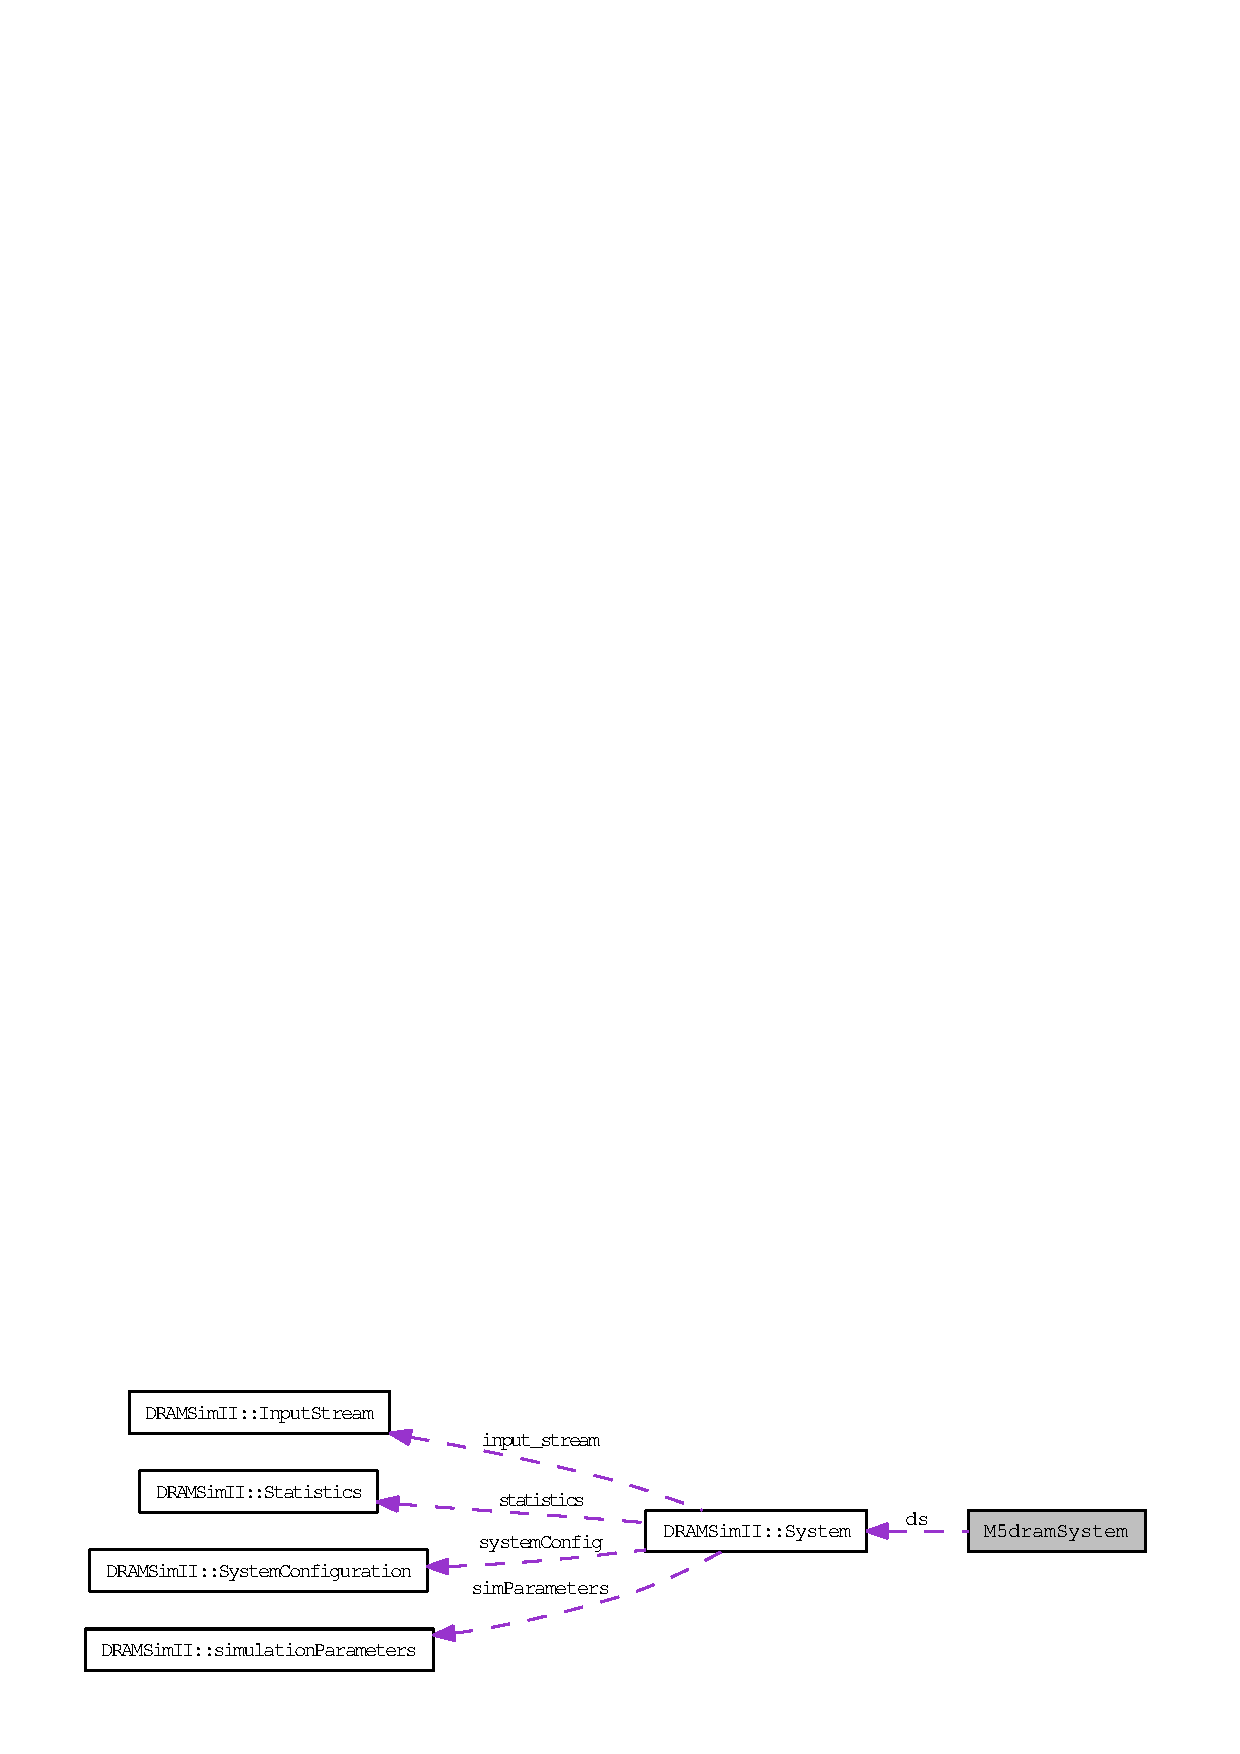
\includegraphics[width=400pt]{class_m5dram_system__coll__graph}
\end{center}
\end{figure}
\subsection*{Public Types}
\begin{CompactItemize}
\item 
typedef M5dramSystemParams {\bf Params}\label{class_m5dram_system_bc049789b7ba009ac06888952383d456}

\begin{CompactList}\small\item\em the parameters used to initialize the memory sytem object \item\end{CompactList}\end{CompactItemize}
\subsection*{Public Member Functions}
\begin{CompactItemize}
\item 
{\bf M5dramSystem} (const {\bf Params} $\ast$)\label{class_m5dram_system_84fc057ba92f2b4259bb6e48dfda6e67}

\begin{CompactList}\small\item\em constructor \item\end{CompactList}\item 
int {\bf getCpuRatio} () const \label{class_m5dram_system_eaafbc3dd2f506366fb2846290519329}

\begin{CompactList}\small\item\em returns the ratio of the cpu frequency to the memory frequency \item\end{CompactList}\item 
float {\bf getInvCPURatio} () const \label{class_m5dram_system_6a265c00d8b099faff4ec0b65b56a69b}

\begin{CompactList}\small\item\em returns the ratio of the memory frequency to the cpu frequency \item\end{CompactList}\end{CompactItemize}
\subsection*{Protected Attributes}
\begin{CompactItemize}
\item 
TickEvent {\bf tickEvent}\label{class_m5dram_system_2c1df40ac4ba1b6ee79a89c36717e6b5}

\begin{CompactList}\small\item\em instance of TickEvent to allow the wrapper to receive/send events to the global queue \item\end{CompactList}\item 
std::vector$<$ MemoryPort $\ast$ $>$ {\bf ports}\label{class_m5dram_system_c74ac86e7c7390068a33e60dfb352427}

\begin{CompactList}\small\item\em ports to send/recv data to other simulator components \item\end{CompactList}\item 
int {\bf lastPortIndex}\label{class_m5dram_system_8dec460f8036d2885f730687e207624c}

\begin{CompactList}\small\item\em the last port accessed \item\end{CompactList}\item 
{\bf DRAMSimII::System} $\ast$ {\bf ds}\label{class_m5dram_system_e4e67af7601cc345bc08d3de8475be65}

\begin{CompactList}\small\item\em pointer to the DRAMSimII class \item\end{CompactList}\item 
bool {\bf needRetry}\label{class_m5dram_system_b1c16d57a7d7a3a07c8c0250be821432}

\begin{CompactList}\small\item\em if the memory system needs to issue a retry statement before any more requests will come in \item\end{CompactList}\item 
unsigned {\bf mostRecentChannel}\label{class_m5dram_system_8f2613214d10b04b640bc26db979484b}

\begin{CompactList}\small\item\em the most recent channel that a request was sent to \item\end{CompactList}\item 
int {\bf cpuRatio}\label{class_m5dram_system_2fbee1e022242e218e235df762bcd82a}

\begin{CompactList}\small\item\em the ratio of the cpu frequency to the memory frequency \item\end{CompactList}\item 
float {\bf invCpuRatio}\label{class_m5dram_system_1411a566b736381786dc016cd805f323}

\begin{CompactList}\small\item\em the ratio of the memory frequency to the cpu frequency \item\end{CompactList}\item 
tick {\bf nextStats}\label{class_m5dram_system_0a3a89735eec2128ba455c89f689a439}

\begin{CompactList}\small\item\em the next time at which stats should be collected \item\end{CompactList}\end{CompactItemize}


\subsection{Detailed Description}
wrapper class to allow M5 to work with DRAMSimII 

The documentation for this class was generated from the following file:\begin{CompactItemize}
\item 
src/m5-dramSystem.h\end{CompactItemize}
